\section{Task 1: First Analysis}
\label{sec:task1}
This section answers assignment Task 3.1 by first converting a fixed barley amount to beer volume and then comparing cost as a function of beer volume for the three fermentable-source routes.

\subsection{Beer Volume from 25.44 kg Barley}
\label{sec:task1-barley-volume}
Using \eqref{eq:barley-to-extract} and \eqref{eq:extract-ratio}, the beer volume obtainable from a barley mass $M_B$ is
\begin{equation}
  \Vbeer
  =0.95\frac{0.6M_B}{2.9(SG-1)}.
  \label{eq:beer-from-barley-task31}
\end{equation}
For $M_B=25.44$ kg, the extract-equivalent mass is $15.264$ kg, the wort volume is $105.269$ L, and the final beer volume is $100.006$ L.

\begin{table}[!t]
\renewcommand{\arraystretch}{1.15}
\caption{Task 1 Barley-to-Beer Calculation}
\label{tab:task31-barley}
\centering
\small
\begin{tabular}{@{}lll@{}}
\toprule
Quantity & Expression & Value \\
\midrule
Barley mass & $M_B$ & 25.44 kg \\
Extract equivalent & $0.6M_B$ & 15.264 kg \\
Wort volume & $0.6M_B/[2.9(SG-1)]$ & 105.269 L \\
Beer volume & $0.95\Vwort$ & 100.006 L \\
\bottomrule
\end{tabular}
\end{table}

\subsection{Cost Functions for Separate Malt-Source Routes}
\label{sec:task1-cost-functions}
The first cost analysis uses the cheapest available barley, malt, malt extract, hops, and yeast from the dataset. With $V$ denoting final beer volume in litres, the separate-route cost functions from \texttt{task\_31.ipynb} are
\begin{align}
  C_{\mathrm{barley}}(V) &= 3482.000 + 0.397529V,\\
  C_{\mathrm{malt}}(V) &= 1072.000 + 0.661836V,\\
  C_{\mathrm{extract}}(V) &= 1.338757V.
\end{align}
The barley route has the largest fixed cost because both malting and mashing are activated. The malt route has only the mashing fixed cost. The malt-extract route has no process fixed cost but has the largest variable cost per litre.

\begin{figure}[!t]
\centering
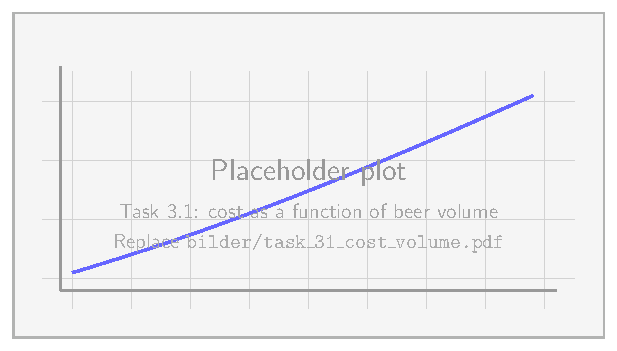
\includegraphics[width=\linewidth]{bilder/task_31_cost_volume}
\caption{Task 1 cost as a function of beer volume. Replace this placeholder with the plot exported from \texttt{task\_31.ipynb}.}
\label{fig:task31-cost-volume}
\end{figure}

\subsection{Combined Malt-Source Solution}
\label{sec:task1-combined}
When all three source routes can be chosen, the combined minimum-cost curve is the lower envelope of the three separate cost curves. For small volumes, malt extract is cheapest because it avoids fixed process costs. For medium volumes, purchased malt becomes cheaper. For large volumes, raw barley becomes attractive because its variable cost per litre is lowest, even though it has the highest fixed process cost.

% Figure \ref{fig:task31-cost-volume}: insert the final plot from task_31.ipynb with the combined curve included.
